\label{forceana}
In setup 3 and setup 4, we stabilised each protein with an external force acting on the FERM domain (see \autoref{motivation}). To ensure that this restraining does not cause major artefacts, the force-dependency of the used observables is examined below.\\
\\
The force has a mean value of $2.44\,\forceunit$ and a standard deviation of $21.80\,\forceunit$. It is skewed to positive values. This is expected since positive values of the force require negative elongations $\Delta z$. If the connecting vector of F1 and F2 $\vec{d}_F$ is parallel to the z-axis the maximal negative elongation is limited by the length of $\vec{d}_F$. Therefore the force would have to stretch the distance between F1 and F2.\\ % TODO: write that this is not so cool with the elastic network?
\\
Linear regressions show that all of the quantities $d_F$, $d_\text{F1-N}$, $d_\text{F2-C}$ and CA have a negligible correlation to the applied force. Here negligible means that either the regression result was not significant or that the obtained slope was so small, that a change of one standard deviations in force would not change the quantity noticeably.\\
\\
We tested also the inter-residue distances for correlation with the applied force. To this end, 10 different proteins without neighbours were picked, each for $1\,\si{\micro\second}$. For each residue pair in this dataset we performed a linear regression. \autoref{force:contactmap} shows the calculated Pearson correlation coefficient (only significant correlations with Pearson $\left|r\right| > 0.3$). The mean value of the slope for the positively correlated pair distances is $33.7\,\si{\pico\newton/\nano\metre}$ and $-32.7\,\si{\pico\newton/\nano\metre}$ for the negatively correlated pair distances. Thus, the force can influence residue pairs contributing to the interface. However, we do not expect major changes in the contact regions, since the majority of residue pairs show only weak correlations.\\
\\
In summary, we do not expect large perturbations of our observables due to the force. However, this approach has limitations. First, there could be e.g. binding poses in multiple FAK interactions requiring a large inclination of the FAK molecule. These states would be suppressed by the force. Another limitation is that, the force does not only prevent tilts around the long axis of FAK (falling to side), but also around the short axis which happens e.g. in FERM-FERM dimers. Lastly the reference to the z-axis is problematically. A reference to the membrane might be better, because it would involve membrane curvature as well. 
%
%
%
\begin{figure}
	\centering
	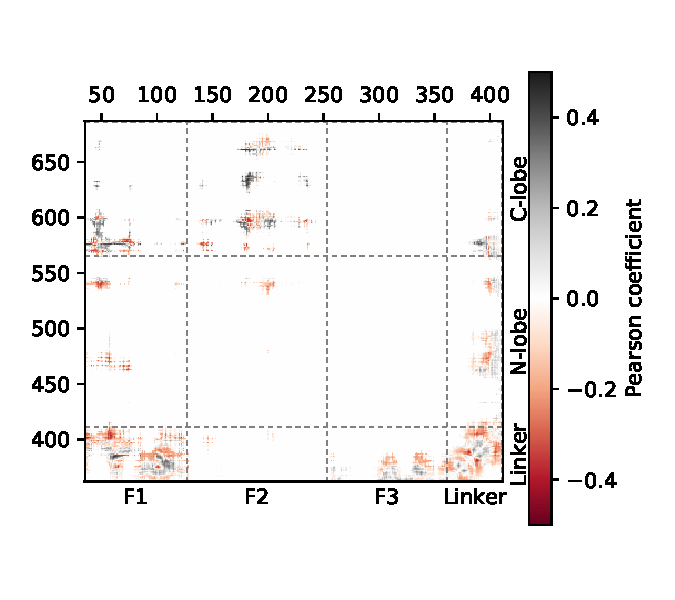
\includegraphics[width=.7\textwidth]{figures/results/interface_corr}
	\nicecaption{Correlations in contact map}{The contact map shows residue pairs whose distance correlates with the applied force.}
	\label{force:contactmap}
\end{figure}
%
%
%